\section{Instalación:}

\subsection{Windows}
 Instalar \href{https://www.python.org/downloads/release/python-368/}{Python 3.6}. Aplicar la opción para añadir a \emph{path}
 Presionando \texttt{[Win]+R} e ingresando \texttt{cmd} accede a la consola. Continuar los pasos en \ref{dep} pero ingresando \ctexttt{python} en lugar de \texttt{python3}.

\subsection{Linux}

\subsubsection{Python 3.6}
\begin{cverbatim}
python3 --version
sudo apt-get update
sudo apt-get install python3.6
\end{cverbatim}
Si no se encuentra:
\begin{cverbatim}
sudo apt-get install software-properties-common
sudo add-apt-repository ppa:deadsnakes/ppa
sudo apt-get update
sudo apt-get install python3.6
\end{cverbatim}

\subsection{Dependencias}\label{dep}

Podemos instalar todas las dependencias usando el \ctexttt{requirements.txt}
\begin{cverbatim}
python3 -m pip install -r requirements.txt
\end{cverbatim}

O por separado:
\begin{cverbatim}
python3 -m pip install pysimplegui
python3 -m pip install playsound
sudo apt-get install python-gst-1.0
python3 -m pip install pattern3.
\end{cverbatim}
\section{Abrir juego:}
Una vez instalado el juego, haga doble click en el archivo \ctexttt{run.py}, y accederá al siguiente menú principal:

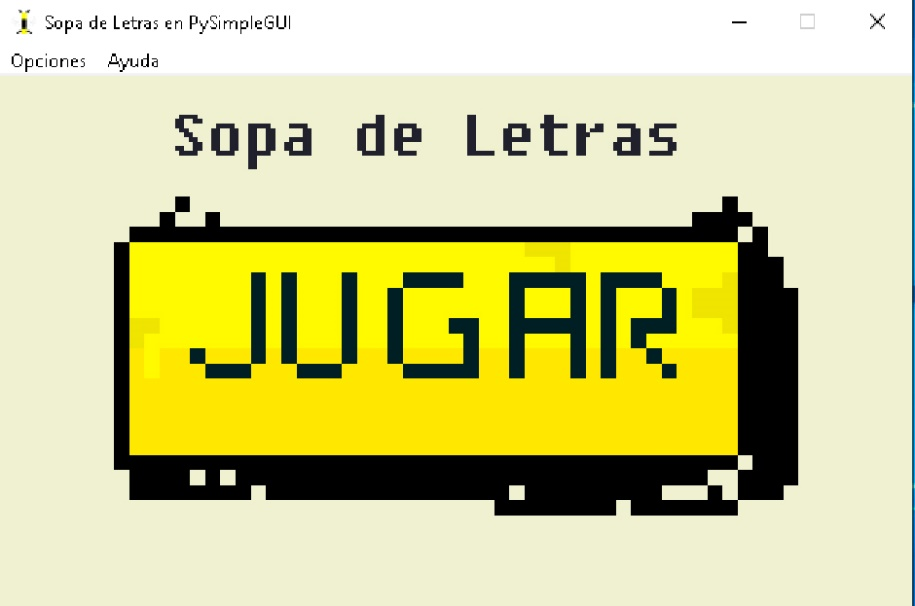
\includegraphics[width=0.8\textwidth,keepaspectratio]{img/guia/1.jpg}

Como la sopa requiere que se carguen las palabras que luego serán exhibidas para que el/la usuario/a las encuentre, la primera vez que ejecute el juego deberá pasar obligadamente por la sección de configuración. Podrá acceder a la misma dirigiéndose al menú de opciones, en la parte superior izquierda de la pantalla. 

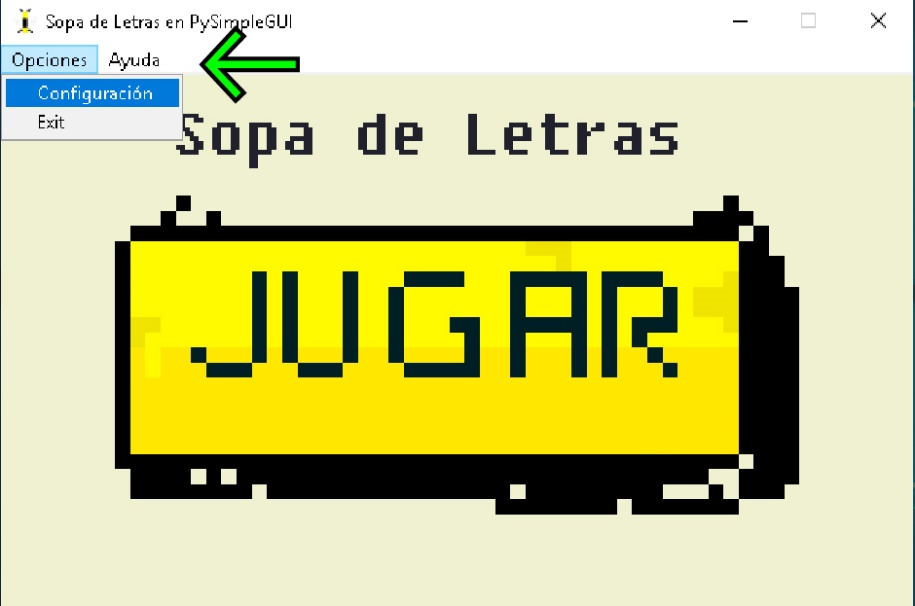
\includegraphics[width=0.8\textwidth,keepaspectratio]{img/guia/2.jpg}

Además de la elección de palabras a buscar, aquí podrá setear una variedad de preferencias, que se detallan a continuación.

\section{Configuración:}
En primer lugar se encuentra la opción de ir introduciendo de a una las palabras que desea que aparezcan en la sopa. Las palabras ingresadas serán verificadas en una base de datos, de la que se obtendrá su definición y su categoría gramatical. En caso de que la palabra ingresada no se halle en la base de datos, se pedirá al/la usuario/a que ingrese la definición correspondiente.

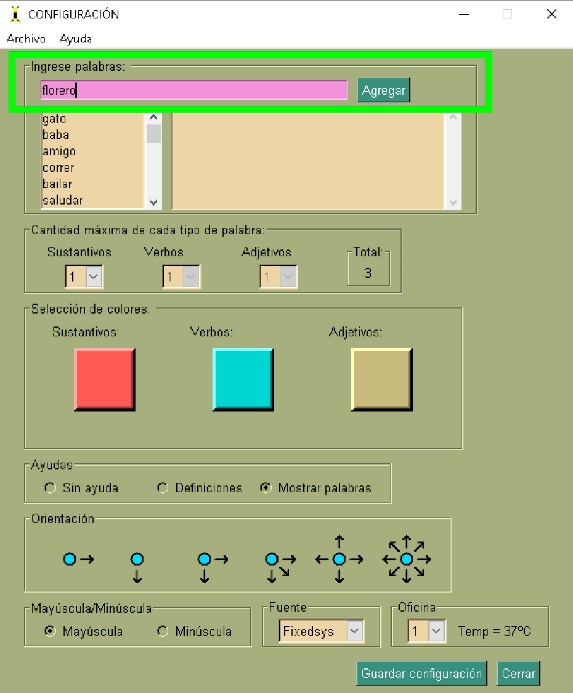
\includegraphics[width=0.6\textwidth,keepaspectratio]{img/guia/3.jpg}

Las palabras que se vayan agregando aparecerán exhibidas en una lista ubicada debajo, de donde se las puede remover haciendo click con el botón derecho sobre la palabra en cuestión, y seleccionando la opción “eliminar” en el menú que se ha desplegado. El menú también ofrece la opción de editar las palabras, o mostrar su definición y categoría gramatical en una nueva ventana. Esta información se muestra también a la derecha de la lista con sólo clickear la palabra en la lista.

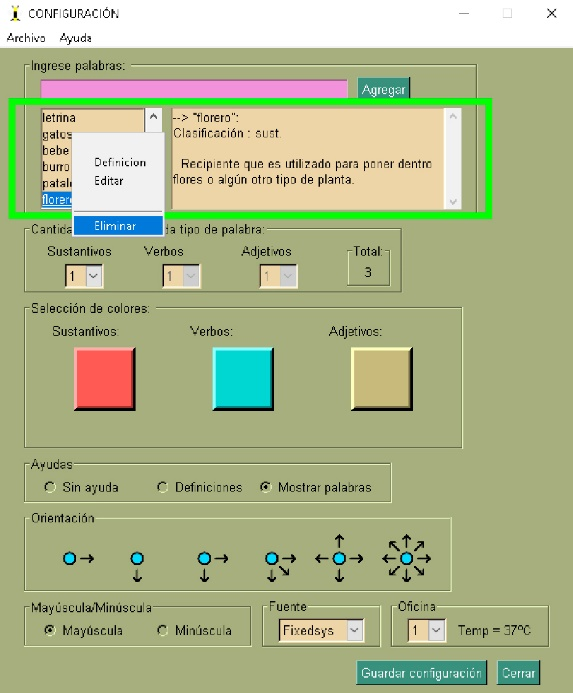
\includegraphics[width=0.6\textwidth,keepaspectratio]{img/guia/5.jpg}

La sopa admite un número máximo de 10 palabras, pero dentro de este límite es posible ajustar la cantidad de palabras con la que desea jugar. La opción “cantidad máxima de cada tipo de palabra” le permite establecer con cuántos sustantivos, cuántos adjetivos y cuántos verbos jugará la próxima partida. (Si la suma de la cantidad de palabras seleccionada en dos categorías supera el máximo, el selector de la categoría restante se bloqueará. Para desbloquearlo, modifique alguno de los primeros (o ambos) hasta que sumen menos de 10.)

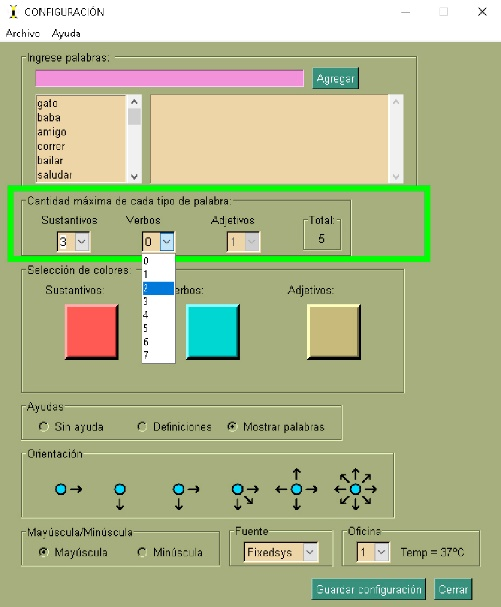
\includegraphics[width=0.6\textwidth,keepaspectratio]{img/guia/6.jpg}

El color del que se marcarán las letras de las palabras encontradas durante el juego dependerá de la categoría gramatical a la que cada palabra pertenezca, y puede ser elegido desde la opción “selección de colores” del menú de configuración. Si los colores seleccionados para dos categorías son demasiado parecidos, se le pedirá cambiar uno de ellos y hasta que no lo haga, no podrá guardar los cambios de configuración ni comenzar el juego.

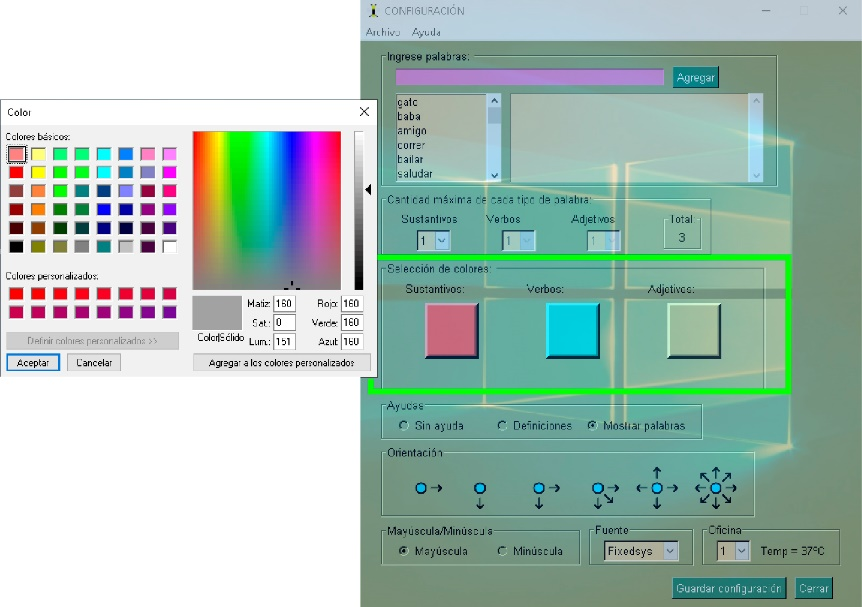
\includegraphics[width=0.9\textwidth,keepaspectratio]{img/guia/7.jpg}

Una de las opciones de configuración que le permitirá variar el grado de dificultad del juego es la opción de ayudas: aquí podrá optar entre jugar sin ayuda, en cuyo caso ni las palabras a encontrar, ni su definición, serán mostradas durante el juego (sólo podrá ver la cantidad de palabras a encontrar); o bien podrá elegir entre dos tipos de ayuda: ver las definiciones de las palabras a encontrar, o simplemente viendo la lista de las palabras ocultas en la sopa seleccionando la opción de mostrar palabras.

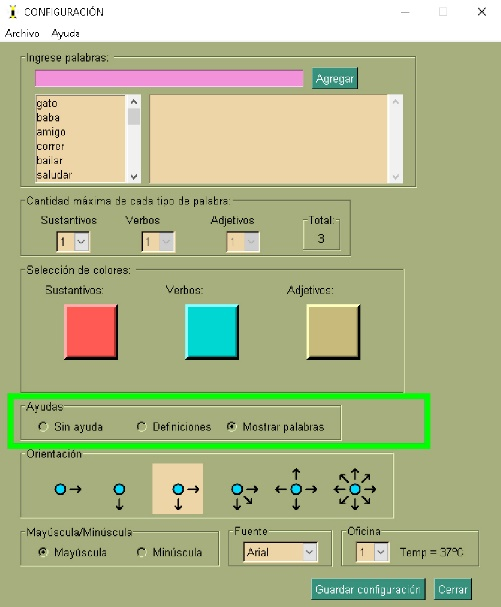
\includegraphics[width=0.6\textwidth,keepaspectratio]{img/guia/8.jpg}
	
Además, se puede conseguir una mayor o menor dificultad en el juego eligiendo entre las distintas opciones de orientación en que las palabras aparecerán dispuestas en la sopa: de izquierda a derecha; de izquierda a derecha y de arriba hacia abajo, etc.

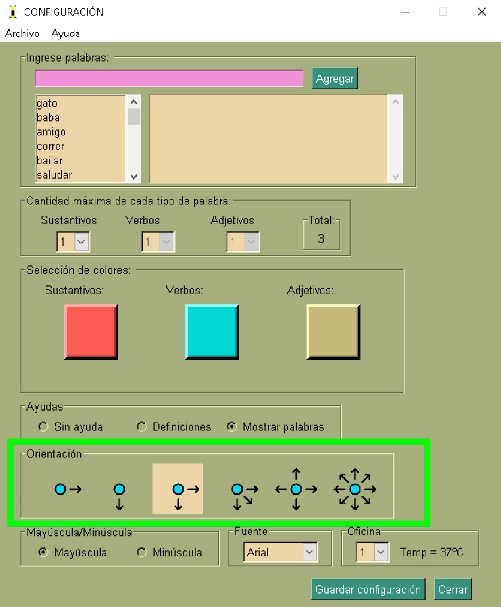
\includegraphics[width=0.6\textwidth,keepaspectratio]{img/guia/9.jpg}

La apariencia del juego puede ser configurada optando entre el uso de letras mayúsculas o minúsculas, y también seleccionando una fuente de entre las varias opciones que el juego incorpora. Por último, el/la usuario/a podrá optar por obtener información de temperatura y humedad y servirse de esta información para configurar la apariencia general del juego, en función de los datos obtenidos por el sensor (raspberry).

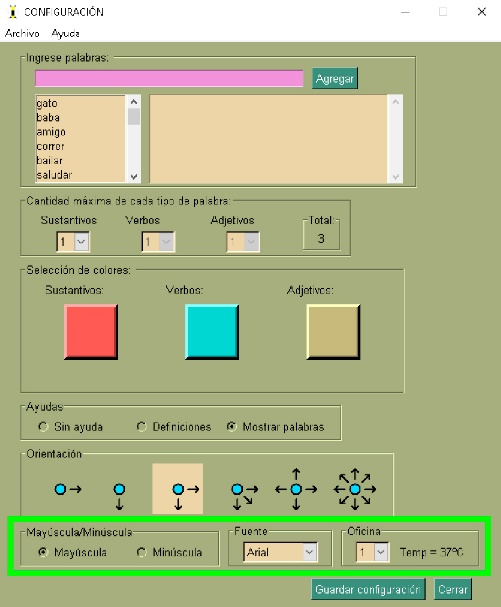
\includegraphics[width=0.6\textwidth,keepaspectratio]{img/guia/10.jpg}

Una vez establecida la configuración del juego según sus preferencias, deberá hacer click en el botón de guardar configuración, situado en la parte inferior derecha de la ventana, y a continuación oprima el botón de cerrar ubicado junto al botón de guardado, para regresar al menú principal, desde donde podrá dar inicio al juego.

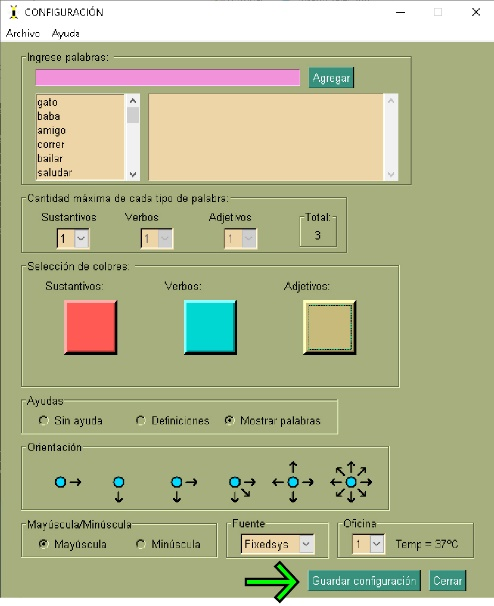
\includegraphics[width=0.6\textwidth,keepaspectratio]{img/guia/11.jpg}

\section{Jugar:}
El juego comenzará cuando oprima el botón “jugar” del menú principal. El objetivo del juego no sólo consiste en encontrar en la sopa la totalidad de las palabras, sino que además se debe marcar cada una de ellas del color correspondiente a su categoría. De manera que antes de empezar a seleccionar una palabra de la sopa, deberá seleccionar el tipo de palabra que va a marcar, oprimiendo alguno de los botones que se encuentran en la parte superior izquierda de la pantalla de juego.

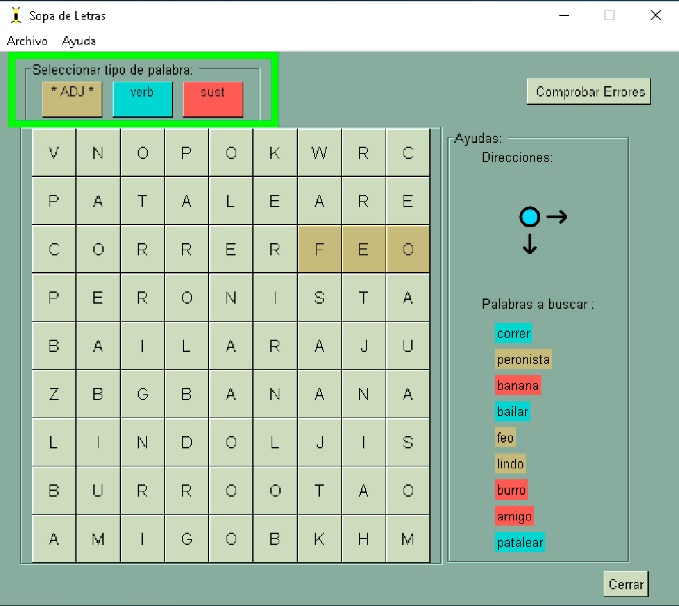
\includegraphics[width=0.8\textwidth,keepaspectratio]{img/guia/12.jpg}

Recuerde que deberá ir cambiando el color del que marcará la palabra a medida que vaya encontrando nuevas palabras de un tipo diferente al último seleccionado.

A la derecha del juego se muestra la información correspondiente a la opción de ayuda seleccionada en la configuración:

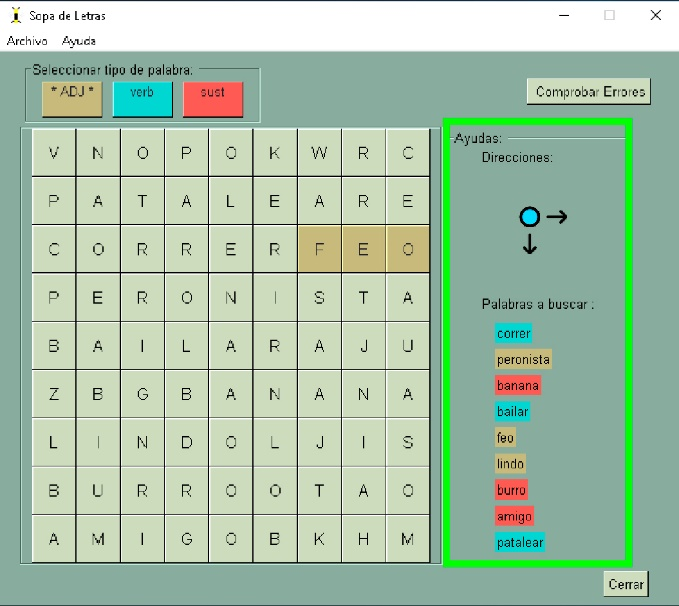
\includegraphics[width=0.8\textwidth,keepaspectratio]{img/guia/13.jpg}

En la esquina superior derecha se encuentra el botón de Comprobar Errores. Al oprimirlo se marcarán en blanco las celdas de letras que hayan sido oprimidas pero no corresponden a ninguna palabra de la lista, o que sí corresponda pero haya sido marcada en un color que no es el que corresponde a la categoría a la que la palabra pertenece.

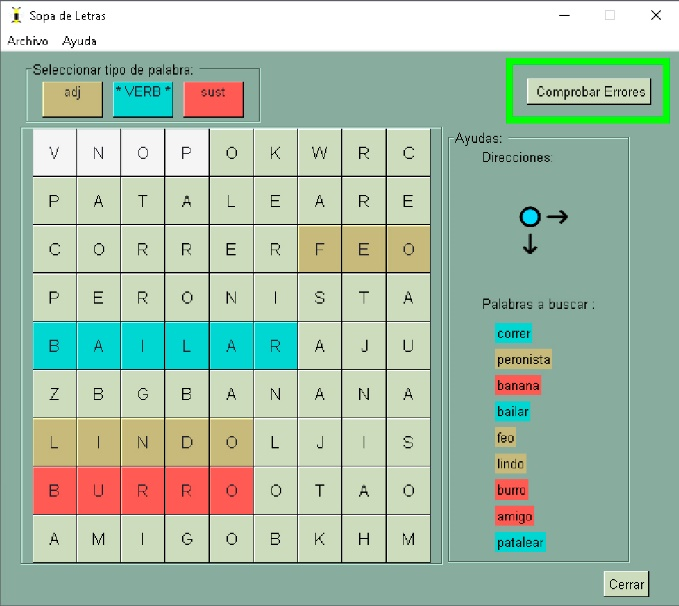
\includegraphics[width=0.8\textwidth,keepaspectratio]{img/guia/14.jpg}

El juego termina cuando la totalidad de las palabras escondidas en la sopa han sido seleccionadas del color adecuado. En ese momento podrá cerrar el juego o volver al menú de configuración y hacer los cambios que desee para volver a jugar.

	

